\chapter{She Turned \$1{,}000 Into a \$66M Empire at 76 Years Old!}

This is a transcript-led chapter. No validated board equations survive from the visual pass, so the mathematics we keep is the mathematics the interview itself insists on: a \$66 million cash exit in a single day, a \$2 million near-sale two years earlier, a \$1{,}000 start, a simple owner-occupant housing identity, a correction from paper rent to collected rent, and a closing rule about beginning with some small but real act of selling. The lecture does not present these as isolated formulas. It unfolds them in order, moving from shock, to persuasion, to timing, and then backward into the conditions that made such an exit possible at all.

\section{Cold Open, Street Recognition, and the \$66 Million Shock}

The lecture begins the way a good problem often begins: with the answer appearing before the method. Barbara Corcoran is stopped on the street, recognized immediately, and asked about money. The host asks for the most she ever made in a year; she answers with a larger correction. It was not a year. It was a day. The resulting quantity is the lecture's first fixed point:
\begin{equation}
V_{\text{exit}}=\$66\,\text{million}.
\end{equation}
The source of that number is equally important. It is not a vague estimate of status. It is the cash outcome from selling the Corcoran Group. Later in the transcript the name is garbled once as ``Corker Group,'' but the referent is plainly the Corcoran Group.

That opening matters because it sets the lecture's rhythm. We are first shown the endpoint, and only then invited to ask how such an endpoint is constructed. The host quickly rewinds the frame, tells us that Barbara is publicly known from \emph{Shark Tank}, reminds us that she is a New York real-estate operator in her own right, and turns the street encounter into a more serious inquiry. The cold open therefore performs a simple structural task: it converts curiosity into permission to examine method.

\section{From Public Persona to Rejection as Advantage}

Once inside the office, the lecture does not rush immediately into doctrine. It spends a few minutes on coats, Shaquille O'Neal, mutual teasing, and Barbara's own admission that she is competitive. That material is not dead air. It tells us, before any theory is offered, what sort of operator is speaking. She is quick, amused, and combative in the productive sense.

Only after that does the host ask the orienting question: what industry did she choose? Barbara's answer is compact and useful: real estate all the way, though \emph{Shark Tank} later exposed her to all kinds of businesses. From there the interview passes naturally into the \emph{Shark Tank} origin story, and now rejection becomes the first real mechanism.

She says she was chosen for the show, signed the contract, was fired, lost the seat, and then regained it before the first day on set. The regain came from persuasion. She wrote a vivid email to the producer, told him he had made a mistake, and reframed the rejection itself as a lucky charm. The lecture's first update rule is therefore not about finance at all. It is about what one does with an adverse signal:
\begin{equation}
\text{rejection}_t \longrightarrow \text{motivation}_{t+1} \longrightarrow \text{assertive response}_{t+2}.
\end{equation}
The point is not that rejection is pleasant. The point is that it need not terminate the process. It can be turned into pressure in the other direction.

This same section plants a second seed. Barbara says she was a phenomenal salesperson and made most of the money in her company that way, but she also says that the real key to getting ahead was delegation. The lecture does not yet stop to unfold that claim, but the order matters. First selling, then scale. First the ability to win the room, then the ability to build a machine larger than oneself.

The Trump anecdote is introduced at exactly this point. Barbara does not present it as moral philosophy. She presents it as a commercial lesson: forceful presentation carries belief with it. She says, bluntly, that she learned from him that people will often buy what is said with confidence, even when it is not delivered in perfectly buttoned-up form. We should preserve that as Barbara Corcoran's heuristic, not as a universal law. But it is the right bridge into the next question, because it sharpens the problem from biography into business mechanism.

\section{Sales, Scarcity, and the Hidden Motivation of the Deal}

The host now asks the lecture's first operational question. Suppose a prospect is on the fence, perhaps leaning no. How do we move the state of the deal?

\subsection{Question \& Answer}

\paragraph{Question.} How do we move a likely no into a yes?

\paragraph{Answer.} Barbara's answer comes in stages. First, do not assume that more talking is the answer. Second, change the structure of the choice. Third, listen hard enough to identify what the buyer is really trying to accomplish.

She says that one of her best tactics was to take the deal away. She would say that someone else had just taken the property, or that there were other offers on it, and the prospect who had been comfortable hesitating would suddenly want it. Scarcity, in her hands, is not a decorative concept. It is a lever that changes the emotional state of the buyer.

We can write her sequence as a simple state diagram:
\begin{figure}[h]
\centering
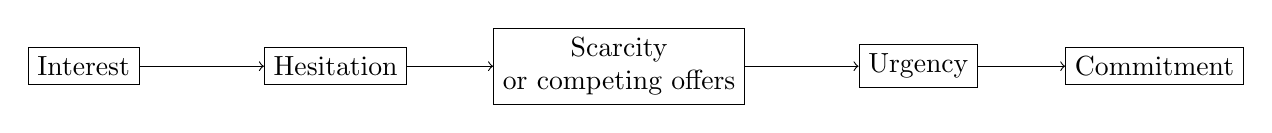
\begin{tikzpicture}
\node[draw, align=center] (a) at (0,0) {Interest};
\node[draw, align=center] (b) at (3.2,0) {Hesitation};
\node[draw, align=center] (c) at (6.8,0) {Scarcity\\or competing offers};
\node[draw, align=center] (d) at (10.6,0) {Urgency};
\node[draw, align=center] (e) at (13.6,0) {Commitment};
\draw[->] (a) -- (b);
\draw[->] (b) -- (c);
\draw[->] (c) -- (d);
\draw[->] (d) -- (e);
\end{tikzpicture}
\caption{Transcript-grounded reconstruction of Barbara Corcoran's negotiation flow. The decisive move is often a change of state rather than an increase in verbal explanation.}
\end{figure}

But the lecture does not stop at scarcity. Barbara immediately adds the deeper point: listening matters more than talking, because the stated desire of the buyer is often not the real motive. This is her rough line about buyers being liars. In more careful notation, the lecture is warning us not to identify observed speech with true motive:
\begin{equation}
M_{\text{stated}} \neq M_{\text{true}}.
\end{equation}

\begin{definition}
The \emph{motivation of a deal} is the operative reason a counterparty will finally move. It is not necessarily the same as the reason first stated aloud.
\end{definition}

Once that distinction is made, her broader negotiation advice becomes easier to read. The harder one listens, the better one can make the deal, because one is no longer guessing blindly. One is trying to infer the hidden variable and then place the right pieces around it. In that cautious sense the lecture's business heuristic is
\begin{equation}
\text{deal success}\approx f(\text{motivation insight},\ \text{urgency},\ \text{timing}).
\end{equation}

The lecture keeps its pace here by moving from a hard saying to a practical instruction. We are not left with ``buyers are liars'' as a slogan. We are shown what the slogan is for. It is for making us listen past surface language and redesign the deal around the real motive.

\section{Timing, Exit Value, and the Same Business at Two Prices}

At this point the lecture loops back to the opening number. The \$66 million line returns, but it now returns under pressure. What was timing doing in that outcome? Barbara first repeats the sale fact, again in the language of a good day and cash in the checking account. Then the host asks the more difficult question.

There is a visible sponsor interruption in the video here. It should not be turned into doctrine. What matters for the notes is that when the interview resumes, it resumes with timing already in the air. Barbara says that she almost sold her business for \$2 million, turned the offer down, and then sold the same business two years later for \$66 million. The comparison is too stark to ignore:
\begin{align}
V_{\text{early}} &= \$2\,\text{million},\\
V_{\text{late}}  &= \$66\,\text{million}.
\end{align}
If we compute only the bare scale comparison, and nothing more ambitious, we obtain
\begin{equation}
\frac{V_{\text{late}}}{V_{\text{early}}}=\frac{66}{2}=33.
\end{equation}

\begin{remark}
The factor \(33\) is only a scale comparison. The transcript gives no earnings, no market multiple, no balance-sheet structure, and no deal terms from which one could derive a formal valuation model. The lecture's actual claim is simpler: timing made an enormous difference to price, even though Barbara describes the underlying business as the same business operating on the same principle.
\end{remark}

A short timeline is enough to capture the logic:
\begin{figure}[h]
\centering
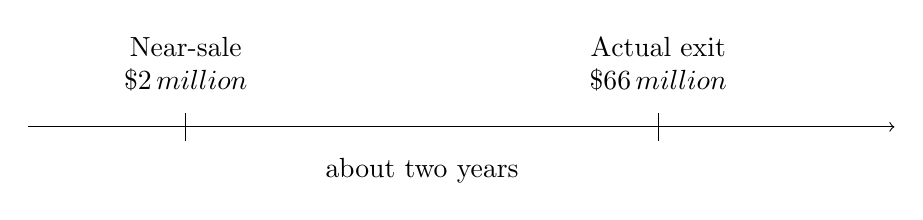
\begin{tikzpicture}
\draw[->] (0,0) -- (11,0);
\draw (2,-0.18) -- (2,0.18);
\draw (8,-0.18) -- (8,0.18);
\node[align=center] at (2,0.8) {Near-sale\\\(\$2\,\text{million}\)};
\node[align=center] at (8,0.8) {Actual exit\\\(\$66\,\text{million}\)};
\node at (5,-0.55) {about two years};
\end{tikzpicture}
\caption{Transcript-grounded timing comparison. The lecture's point is not a formal return calculation but a sharp contrast in realized price across time.}
\end{figure}

What is striking is Barbara's refusal to mystify the answer. When the host asks what she saw in the market that told her to wait, she says, in effect, that she wanted more money. If someone had offered her \$66 million then, she would have sold then. That answer keeps the chapter honest. Timing matters, but the lecture does not derive timing from some hidden macroeconomic oracle. It treats timing as part of commercial judgment, and in this case part of bargaining over value.

\section{Real Estate Formula: Vision, Residential Demand, and Getting in Early}

Only after the lecture has shown us the exit and its timing does it walk backward to the beginning. The host now reminds us that Barbara started with a thousand-dollar loan:
\begin{equation}
C_0=\$1{,}000.
\end{equation}
Asked for her formula, she begins not with analysis but with vision. She says she saw herself as the queen of New York real estate, could see it in living color, could almost touch it, and carried that image as a guide. In these notes we should not dismiss that as decoration. In the lecture it functions as a stabilizing condition on action. Long before a proof exists, the operator has chosen the direction in which she expects reality to bend.

The host then pushes on self-belief. Barbara's answer is revealingly unsentimental. She had held many jobs. If this one failed, she could get another. She was, by her own description, happy poor. In other words, self-belief here is not presented as mystical self-esteem. It is partly built out of a low catastrophe estimate. Failure would hurt, but it would not end the world.

The next move is from psychology to asset class. Why residential? Because, she says, people need a place to live. Through highs and lows in New York, that need persists. The lecture's structural claim about real estate is therefore extremely plain, and for that reason durable: necessity places a floor under demand.

\subsection{Question \& Answer}

\paragraph{Question.} What was the formula for accumulating wealth in real estate?

\paragraph{Answer.} The lecture gives the formula in layers. Hold a vivid long-run picture. Choose a segment with persistent demand. Enter early enough that time can work in your favor. If capital is limited, structure the first property so that somebody else helps carry the asset.

That last point is stated with unusual concreteness. Barbara says that if a young person had around \$100{,}000 to put to work, she would put it into a two-family house, live in one unit, and let the other tenants pay rent and help pay off the mortgage. The transcript garbles one phrase here, but the economic structure is plain. In cleaned notation:
\begin{equation}
C_{\text{owner,net}}
=
C_{\text{mortgage}}+C_{\text{tax}}+C_{\text{upkeep}}-R_{\text{second unit}}.
\end{equation}
This is only a schematic identity. The lecture supplies no interest rate, tax bill, purchase price, or maintenance schedule. But the identity is exactly the right level of abstraction for what Barbara is saying: the first asset is easier to enter when occupancy and rent are combined.

\begin{figure}[h]
\centering
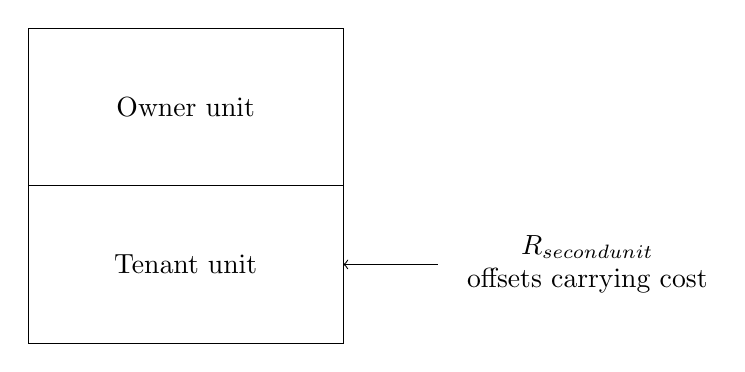
\begin{tikzpicture}
\draw (0,0) rectangle (4,4);
\draw (0,2) -- (4,2);
\node at (2,3) {Owner unit};
\node at (2,1) {Tenant unit};
\draw[->] (5.2,1) -- (4,1);
\node[align=center] at (7.1,1) {\(R_{\text{second unit}}\)\\offsets carrying cost};
\end{tikzpicture}
\caption{Transcript-grounded reconstruction of the two-family-house strategy. One lives in one unit and uses rent from the other to reduce the effective housing burden.}
\end{figure}

The lecture immediately couples this with a warning about delayed entry. Barbara says she tried to buy a Greenwich Village studio at twenty-seven, became scared, and deliberately failed the board. It then took her about eight years to catch up to the market:
\begin{equation}
\Delta t_{\text{lost}}\approx 8\ \text{years}.
\end{equation}
That is one of the chapter's cleanest numerical lessons. Delay has a cost, and in this case the cost is not an abstract opportunity cost but an entire segment of market movement that slipped out of reach.

\section{Concentration, Founder Selection, and Paper Wealth versus Real Cash Flow}

The lecture now broadens from one asset class to business judgment more generally. The host offers the familiar slogan that concentration builds wealth and diversification keeps it. Barbara does not accept the slogan as a rule for herself. She says she invests in many kinds of businesses, but what she really judges is the entrepreneur. The center of gravity therefore shifts from category to operator.

A concise reconstruction of her investment screen is
\begin{equation}
Q_{\text{investment}}
\approx
f(\text{resilience},\ \text{sales ability},\ \text{judgment},\ \text{fire-in-the-belly}).
\end{equation}
The lecture sharpens this screen when Barbara says that the difference between good people and phenomenal people is the ability to get back up. She then widens the list: entrepreneurs must be able to sell, judge people, make calls, and have business acumen. In the lecture's logic, the founder is not an ornament attached to the business. The founder is one of the principal variables.

Two small but important transitions occur here. First, when asked what industry she would enter if starting over, Barbara answers not with sector rotation or a trend chart but with something she loved. She even says she would try the flower business. Second, when asked whether the key trait can be learned, she gives a mixed answer: some of it can be developed or exaggerated, but not all of it is evenly distributed. The point is not to resolve that nature-versus-cultivation debate fully. The point is that the lecture treats passion, resilience, and commercial temperament as live components of expected business quality.

The motel story then provides the chapter's strongest paper-versus-reality example. Barbara says she bought a 12-unit motel. On paper it had a juicy rent roll. In reality, once she became owner, she discovered that nobody had paid rent in two years. This is the exact place where a note-writer should stop trusting nominal description and write down the correction:
\begin{equation}
R_{\text{collected}}=R_{\text{scheduled}}\times \rho_{\text{collection}}.
\end{equation}
Here the dramatic fact of the anecdote is that \(\rho_{\text{collection}}\) was effectively near zero despite the attractive paper presentation. The rent roll looked like income. It was not income.

That lesson belongs alongside the earlier sales lesson. Just as stated buyer preference is not the same as true motive, paper revenue is not the same as cash collected. Again and again the lecture teaches us to distrust the surface and look for the operative variable beneath it.

Barbara ends this stretch by refusing to sentimentalize loss. She says she always loses money and does not care in isolation. It is a long game. The important distinction is not between perfect winners and flawed losers, but between people who stay in motion and people who cannot survive the oscillation of gain and error.

\section{Doubt, Authenticity, and the Closing Rule of Action}

The last movement of the lecture becomes broader and faster, but it still follows the same underlying logic. It begins with a practical geographic answer. If starting a first business today, Barbara says, she might go to Pittsburgh: young people, incoming medical and technology activity, and a government friendly to landlords. The answer is not mathematical in form, but it is still a judgment about where opportunity clusters.

Then the subject becomes doubt. Barbara says she was doubted from the start: by the old boys' club, by Donald Trump, by Mark Burnett. A sharp numerical marker remains attached to the Trump story, namely the threatened denial of a commission:
\begin{equation}
\Pi_{\text{commission}}=\$4\,\text{million}.
\end{equation}
The transcript around one phrase in that anecdote is unstable, but the economic point is firm enough. Doing the deal is not always the end of the struggle; one may still have to fight to secure the value one created.

This is why the earlier rejection logic returns here in more explicit form. Barbara says that the minute doubt appears, one should use it for motivation and push ahead:
\begin{equation}
\text{doubt}\longrightarrow \text{motivation}\longrightarrow \text{push ahead}.
\end{equation}
That line links the \emph{Shark Tank} recovery story to the late-career reflections. Rejection is not only an early-career accident. It is part of the permanent operating environment.

The lecture then turns, quickly but not accidentally, to partner choice, school performance, communication, and authenticity. Barbara says that a good life partner or business partner doubles one's chances of success. The phrase should be heard as emphatic causal language, not as an actuarial estimate, but the claim itself is clear: the people nearest us change the odds of what we can sustain. She says her grades did not amount to much, that one can use one's mouth or whatever asset one has, and that her own fear may have helped push her forward. She also says that not having affluent parents made her freer, because she did not have to preserve somebody else's image of what her life should look like.

All of that converges on authenticity. Barbara says that once she became herself, stopped trying to fit a fancy mold, and built on what she already had, things moved more cleanly.

\subsection{Question \& Answer}

\paragraph{Question.} If we had to start from zero, what is the first move?

\paragraph{Answer.} Barbara refuses the grandiose formulation of the problem. Asked what she would do if she had one year to make a million dollars and her life depended on it, she says she would not begin by planning a million-dollar year. She would begin by selling apples on the corner, making about \$50{,}000 in the first month, and building from there.

In the notation of these notes:
\begin{equation}
R_{\text{month 1, apples}}\approx \$50{,}000.
\end{equation}
The point is not that apples are a hidden universal business model. The point is that motion begins with something real, immediate, and saleable. The lecture's final advice is therefore not to fantasize about terminal wealth, but to generate early cash flow and let reinvestment take over from there.

\section{Summary}

The chapter begins, as the lecture begins, with a number that is too large to ignore and then spends the rest of its time earning that number. The \$66 million exit is not left standing alone. It is connected to persuasion under rejection, to scarcity and listening in sales, to a dramatic timing contrast with an earlier \$2 million near-sale, to a \$1{,}000 beginning in residential real estate, to a two-family-house entry structure, to a correction from paper rent to actual collections, and finally to a rule of starting from zero by selling something real.

What survives the interview's speed is a compact set of mechanisms. Surface statements are not always the true variable. Timing changes value. Housing demand has a stubborn baseline. Founder quality can dominate category. Doubt can be converted into forward motion. And when the question becomes how to begin, the lecture answers in the simplest possible way: begin with action, begin with sales, and let the mathematics of accumulation start there.